\documentclass[12pt]{article}
\usepackage{amsmath}
\usepackage{amssymb}
\usepackage{listings}
\usepackage{framed}
\usepackage{graphicx}
\usepackage{algorithm}
\usepackage{algorithmicx}
\usepackage{algpseudocode}

\author{Sean White, Kierstyn Brandt, Rostik Mertz, Norman Tang}
\title{CSCI 432 - Project Deliverable 5}

\begin{document}
\maketitle

For this paper we are examining the convex hull algorithm created by Timothy Chan in 1996. This algorithm takes $n$ points on a graph and seeks to create the smallest possible polygon that encloses all points. We will derive the asymptotic upper bound of the worst case runtime of this algorithm, then compare it to the mini-ball algorithm covered in class as they solve similar problems. We will then look at what is known as the \textit{aspect ratio}, which is defined as the area of the washer created between the smallest enclosing ball (mini-ball) and the largest inscribing circle and compare the runtime to finding the area of the polygon created by the convex hull.

So far we have pseudocode for convex hull, mini-ball, and largest inscribing circle, as well as runtimes for each. We will not include those here for the sake of space, as this report must be under 2 pages the pseudocode would take this up on their own. Next we will write out proofs for each upper bound, find algorithms for the area of the convex hull and aspect ratio, and find some way to compare results. then we will implement these algorithms and generate a set of points to run them on to test. 

Since the video must revolve around our +1 as required by the assignment, we are discussing different ways to visualize the two algorithms side by side. The obvious answer would be to create a program that shows the convex hull algorithm and mini-ball algorithm running side by side, but this would be short and, in our opinion, somewhat bland. So, we will feature this, but it cannot be the only thing we do in the video. One idea we had was to extend the video by running this comparison on multiple datasets with different features. Some sparse, some dense, some large, some small, so on and so forth and then report on our findings on how each algorithm handled these edge cases.

One feature can compare the algorithms is to look at how the aspect ratios differ given these edge cases, since we suspect that for a number of these edge cases that the running time may not actually differ enough in appreciable amounts. We also found ways to figure out the area of the polygons of the convex hull, which is a little more complicated then the taking the area of the enclosing ball and the largest inscribing circle. Some interesting cases may possibly comparing a data set that looks like a square against one that forms a circle. Other ideas were to compare one large grouping with a loner point, and two distinct groupings together.

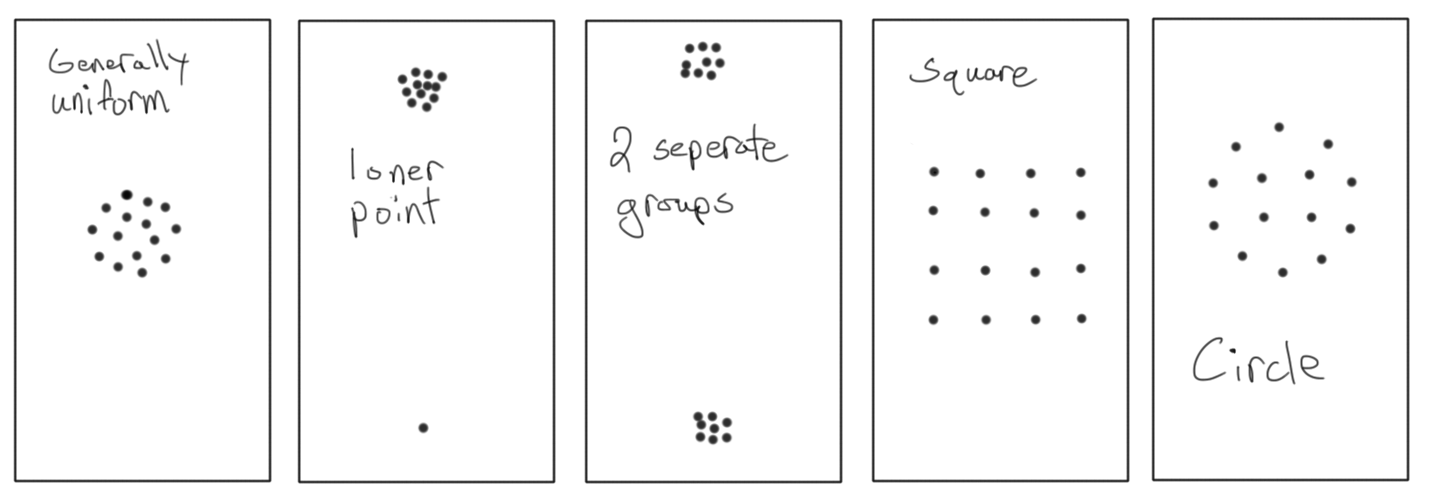
\includegraphics[width=\textwidth]{EdgeCases.png}

\end{document}